% ============================================================
%   EPSS-TPG training and testing context (two-column figure)
% ============================================================
%
% Companion to model_architecture_abstract.tex. The architecture
% figure shows the per-CVE model; this figure shows how the same
% model is used across the full lifecycle (data preparation,
% training loop with validation, testing on a held-out split).
%
% The page is sized close to the figure bounding box, so when
% imported via \includegraphics[width=\linewidth]{...} into a
% two-column paper it scales to the column width without extra
% white space.
%
% Compile:
%   pdflatex -interaction=nonstopmode training_testing_context.tex
% ============================================================

\documentclass[10pt]{article}

\usepackage[paperwidth=310mm, paperheight=175mm, margin=4mm]{geometry}
\usepackage{tikz}
\usepackage{amsmath}
\usepackage{amssymb}
\pagestyle{empty}

\usetikzlibrary{positioning, arrows.meta, calc, fit, backgrounds}

% Colour palette in the same family as the architecture diagram.
\definecolor{cData}{RGB}{236,244,255}      % data prep  (light blue)
\definecolor{cTrain}{RGB}{223,239,223}     % training   (light green)
\definecolor{cVal}{RGB}{255,247,210}       % validation (light yellow)
\definecolor{cCkpt}{RGB}{229,229,229}      % checkpoint (light grey)
\definecolor{cTest}{RGB}{255,236,217}      % testing    (light orange)
\definecolor{cMetric}{RGB}{255,222,222}    % metrics    (light pink)
\definecolor{cModel}{RGB}{217,237,237}     % model      (light teal)
\definecolor{accent}{RGB}{20,70,140}

\tikzset{
    box/.style={
        rectangle, rounded corners=2pt, draw=black!55,
        line width=0.45pt, inner sep=4pt,
        align=center, font=\small,
        minimum height=14mm, minimum width=28mm,
    },
    boxwide/.style={box, minimum width=38mm},
    boxsmall/.style={
        rectangle, rounded corners=2pt, draw=black!55,
        line width=0.45pt, inner sep=3pt,
        align=center, font=\scriptsize,
        minimum height=11mm, minimum width=26mm,
    },
    model/.style={
        rectangle, rounded corners=2pt, draw=accent, fill=cModel,
        line width=0.7pt, inner sep=4pt,
        align=center, font=\small\sffamily,
        minimum height=14mm, minimum width=30mm,
    },
    flow/.style={
        -{Stealth[length=2.5mm]}, line width=0.55pt, draw=black!75
    },
    feedback/.style={
        -{Stealth[length=2mm]}, line width=0.5pt, draw=accent!85, dashed
    },
    bandlabel/.style={
        font=\sffamily\bfseries\small, text=accent, align=center
    },
    edgelab/.style={
        font=\scriptsize, text=black!60, inner sep=1pt, align=center
    },
}

\begin{document}

\noindent
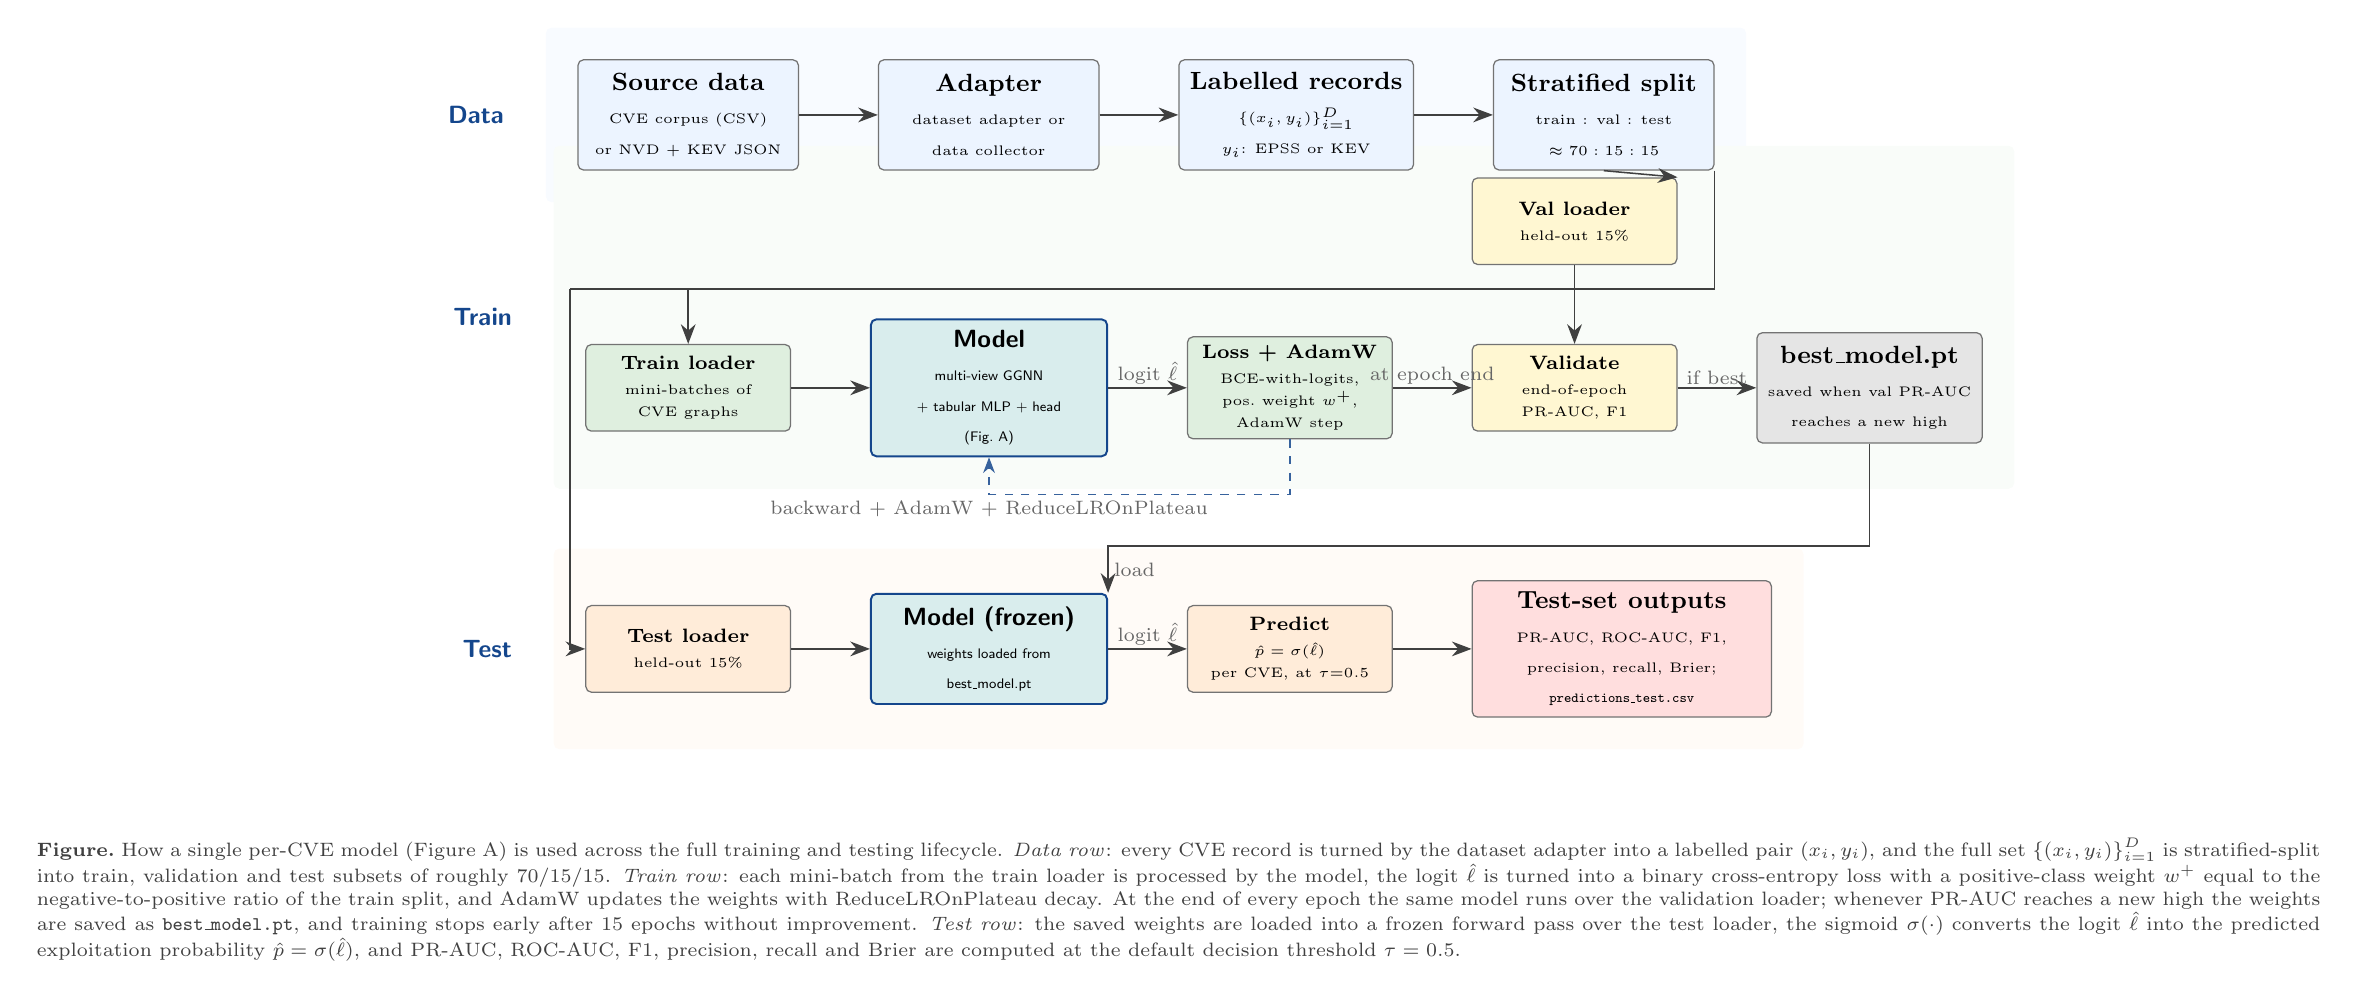
\begin{tikzpicture}[node distance=12mm and 10mm]

% ============================================================
%   ROW 1 - DATA PREPARATION
% ============================================================

\node[box, fill=cData] (raw) {
    \textbf{Source data}\\[1pt]
    {\tiny CVE corpus (CSV)}\\
    {\tiny or NVD + KEV JSON}
};

\node[box, fill=cData, right=of raw] (adapter) {
    \textbf{Adapter}\\[1pt]
    {\tiny dataset adapter or}\\
    {\tiny data collector}
};

\node[box, fill=cData, right=of adapter] (lab) {
    \textbf{Labelled records}\\[1pt]
    {\tiny $\{(x_i, y_i)\}_{i=1}^{D}$}\\
    {\tiny $y_i$: EPSS or KEV}
};

\node[box, fill=cData, right=of lab] (split) {
    \textbf{Stratified split}\\[1pt]
    {\tiny train : val : test}\\
    {\tiny $\approx 70 : 15 : 15$}
};

\draw[flow] (raw)     -- (adapter);
\draw[flow] (adapter) -- (lab);
\draw[flow] (lab)     -- (split);

% ============================================================
%   ROW 2 - TRAINING LOOP
%   One clean horizontal flow:
%      Train loader -> Model -> Loss + AdamW -> Validate -> best_model.pt
%   Plus:
%      Val loader sits above Validate and feeds it.
%      A dashed feedback arrow loops Loss back into Model
%      (backward pass + optimiser step + LR scheduler).
% ============================================================

\node[boxsmall, fill=cTrain, below=22mm of raw] (trainld) {
    \textbf{Train loader}\\[1pt]
    {\tiny mini-batches of}\\
    {\tiny CVE graphs}
};

\node[model, right=of trainld] (modelTr) {
    \textbf{Model}\\[1pt]
    {\tiny multi-view GGNN}\\
    {\tiny + tabular MLP + head}\\
    {\tiny (Fig.~A)}
};

\node[boxsmall, fill=cTrain, right=of modelTr] (loss) {
    \textbf{Loss + AdamW}\\[1pt]
    {\tiny BCE-with-logits,}\\
    {\tiny pos.\ weight $w^+$,}\\
    {\tiny AdamW step}
};

\node[boxsmall, fill=cVal, right=of loss] (valeval) {
    \textbf{Validate}\\[1pt]
    {\tiny end-of-epoch}\\
    {\tiny PR-AUC, F1}
};

\node[box, fill=cCkpt, right=of valeval] (best) {
    \textbf{best\_model.pt}\\[1pt]
    {\tiny saved when val PR-AUC}\\
    {\tiny reaches a new high}
};

% Val loader sits above Validate and feeds it.
\node[boxsmall, fill=cVal, above=10mm of valeval] (valld) {
    \textbf{Val loader}\\[1pt]
    {\tiny held-out 15\%}
};

\draw[flow] (valld) -- (valeval);

% Main forward flow along Row 2.
\draw[flow] (trainld) -- (modelTr);
\draw[flow] (modelTr) -- node[edgelab, midway, above]
    {logit $\hat{\ell}$} (loss);
\draw[flow] (loss)    -- node[edgelab, midway, above]
    {at epoch end} (valeval);
\draw[flow] (valeval) -- node[edgelab, midway, above]
    {if best} (best);

% Single feedback arrow: Loss step updates Model weights.
\draw[feedback] (loss.south) -- ++(0,-7mm) -| (modelTr.south)
    node[edgelab, midway, below=1pt]
    {backward $+$ AdamW $+$ ReduceLROnPlateau};

% Split feeds all three loaders. The val loader sits directly
% under split (it occupies split's x-column), so a naive vertical
% drop from split.south would pass through valld. We instead use:
%   - a short diagonal from split.south to valld.north east for
%     the val loader, and
%   - a plain stem dropped from split's south-east corner (outside
%     valld's x-range) that runs left at y = -22 (below valld but
%     above row 2) with branch arrows down to trainld and testld.
% This removes every box-piercing or overlapping segment.

\coordinate (stemDown) at ([yshift=-15mm]split.south east);
\coordinate (stemLeft) at ([xshift=-15mm]trainld.north |- stemDown);

% Plain stem (no arrowhead) carrying both the train and test feeds.
\draw[line width=0.55pt, draw=black!75]
    (split.south east) -- (stemDown) -- (stemLeft);

% Val loader: short diagonal arrow, clear of all other elements.
\draw[flow] (split.south) -- (valld.north east);

% Train loader: branch arrow dropping from the stem.
\draw[flow] (trainld.north |- stemDown) -- (trainld.north);

% ============================================================
%   ROW 3 - TESTING
% ============================================================

\node[boxsmall, fill=cTest, below=22mm of trainld] (testld) {
    \textbf{Test loader}\\[1pt]
    {\tiny held-out 15\%}
};

\node[model, right=of testld] (modelTe) {
    \textbf{Model (frozen)}\\[1pt]
    {\tiny weights loaded from}\\
    {\tiny best\_model.pt}
};

\node[boxsmall, fill=cTest, right=of modelTe] (predict) {
    \textbf{Predict}\\[1pt]
    {\tiny $\hat p = \sigma(\hat{\ell})$}\\
    {\tiny per CVE, at $\tau{=}0.5$}
};

\node[boxwide, fill=cMetric, right=of predict] (metrics) {
    \textbf{Test-set outputs}\\[1pt]
    {\tiny PR-AUC, ROC-AUC, F1,}\\
    {\tiny precision, recall, Brier;}\\
    {\tiny \texttt{predictions\_test.csv}}
};

% Test loader: branch arrow continuing down from the left end of
% the stem (defined in the training block above). The vertical at
% x = stemLeft.x is left of trainld's left edge, so it does not
% pierce trainld on its way down to row 3.
\draw[flow] (stemLeft) |- (testld.west);

% Checkpoint loads into the test model. Routed so it does NOT
% overlap the dashed feedback loop. The feedback loop occupies
% y in [-48.5, -41.5] at x = 38 (modelTr.x = modelTe.x), so we
% drop best.south below that band (down 13mm to y = -54.5),
% travel left, then come up into modelTe.north east. Entering on
% the east edge avoids the x=38 vertical entirely.
\draw[flow] (best.south) -- ++(0,-13mm) -| (modelTe.north east)
    node[edgelab, near end, right=1pt] {load};

% Forward pass on test data.
\draw[flow] (testld)  -- (modelTe);
\draw[flow] (modelTe) -- node[edgelab, midway, above]
    {logit $\hat{\ell}$} (predict);
\draw[flow] (predict) -- (metrics);

% ============================================================
%   Band groupings behind the rows
% ============================================================
\begin{scope}[on background layer]
    \node[fit=(raw)(adapter)(lab)(split), inner sep=4mm,
          fill=cData!35, rounded corners=2pt] (bandData) {};
    \node[fit=(trainld)(modelTr)(loss)(valld)(valeval)(best),
          inner sep=4mm,
          fill=cTrain!18, rounded corners=2pt] (bandTrain) {};
    \node[fit=(testld)(modelTe)(predict)(metrics),
          inner sep=4mm,
          fill=cTest!22, rounded corners=2pt] (bandTest) {};
\end{scope}

\node[bandlabel, left=4mm of bandData.west]  {Data};
\node[bandlabel, left=4mm of bandTrain.west] {Train};
\node[bandlabel, left=4mm of bandTest.west]  {Test};

% ============================================================
%   Caption (below the figure). Kept inside the standalone
%   bounding box so the figure is self-contained when viewed
%   on its own. When the figure is included in a paper via
%   \includegraphics{}, prefer the suggested \caption{...}
%   block reproduced as a comment at the end of this file.
% ============================================================
\node[font=\scriptsize, text=black!75, text width=290mm,
      align=justify, anchor=north]
      (cap) at ($(bandTest.south)+(0,-1.0cm)$) {%
    \textbf{Figure.}\ How a single per-CVE model (Figure~A)
    is used across the full training and testing lifecycle.
    \emph{Data row}: every CVE record is turned by the
    dataset adapter into a labelled pair $(x_i, y_i)$, and
    the full set $\{(x_i, y_i)\}_{i=1}^{D}$ is
    stratified-split into train, validation and test subsets
    of roughly 70/15/15. \emph{Train row}: each mini-batch
    from the train loader is processed by the model, the
    logit $\hat\ell$ is turned into a binary cross-entropy
    loss with a positive-class weight $w^+$ equal to the
    negative-to-positive ratio of the train split, and
    AdamW updates the weights with ReduceLROnPlateau decay.
    At the end of every epoch the same model runs over the
    validation loader; whenever PR-AUC reaches a new high
    the weights are saved as \texttt{best\_model.pt}, and
    training stops early after 15 epochs without
    improvement. \emph{Test row}: the saved weights are
    loaded into a frozen forward pass over the test loader,
    the sigmoid $\sigma(\cdot)$ converts the logit
    $\hat\ell$ into the predicted exploitation probability
    $\hat p = \sigma(\hat\ell)$, and PR-AUC, ROC-AUC, F1,
    precision, recall and Brier are computed at the default
    decision threshold $\tau = 0.5$.
};

\end{tikzpicture}

\end{document}

% ============================================================
%   Suggested figure caption for paper integration
% ============================================================
%
% Copy this into a \begin{figure*}...\end{figure*} block:
%
% \begin{figure*}[t]
%   \centering
%   
\includegraphics[width=\linewidth]{training_testing_context}
%   \caption{How a single per-CVE model (Fig.~A) is used
%   across the full training and testing lifecycle, with
%   weights frozen at test time.
%   \textbf{Data} (top): every CVE record is turned by the
%   dataset adapter into a labelled pair $(x_i, y_i)$, where
%   $x_i$ is the per-CVE input (text plus tabular metadata)
%   and $y_i$ is the training target (the EPSS score for
%   soft-label runs, KEV membership for binary runs). The
%   full set $\{(x_i, y_i)\}_{i=1}^{D}$ is stratified-split
%   into train, validation and test subsets of roughly
%   70/15/15.
%   \textbf{Train} (middle): each mini-batch from the train
%   loader is processed by the multi-view GGNN plus tabular
%   branch of Fig.~A. The model emits a logit
%   $\hat{\ell}$, which the loss head turns into a binary
%   cross-entropy term with a positive-class weight $w^+$
%   equal to the negative-to-positive ratio of the train
%   split, minimised by AdamW with gradient clipping at
%   $1.0$ and learning rate $10^{-3}$. At the end of every
%   epoch the same model runs over the validation loader;
%   whenever PR-AUC reaches a new high the weights are
%   saved to \texttt{best\_model.pt}. The learning rate is
%   decayed by ReduceLROnPlateau (mode max, factor $0.5$,
%   patience $5$, minimum $10^{-6}$) and training stops
%   early after $15$ epochs without a validation PR-AUC
%   improvement.
%   \textbf{Test} (bottom): the frozen weights are loaded
%   from \texttt{best\_model.pt} into a fresh forward pass
%   over the test loader; the sigmoid $\sigma(\cdot)$
%   converts the logit $\hat{\ell}$ into the predicted
%   exploitation probability $\hat{p} = \sigma(\hat{\ell})$.
%   PR-AUC, ROC-AUC, F1, precision, recall and Brier are
%   computed at the default decision threshold
%   $\tau = 0.5$ and per-CVE predictions are written to
%   \texttt{predictions\_test.csv}.
%   \textit{Variables:}
%   $x_i$, per-CVE input;
%   $y_i$, training target;
%   $D$, size of the labelled dataset;
%   $\hat{\ell}$, model logit;
%   $\hat{p} = \sigma(\hat{\ell})$, predicted probability;
%   $w^+$, positive-class weight;
%   $\tau$, decision threshold;
%   $g \in \mathbb{R}^{256}$, graph-level vector (Fig.~A);
%   $t \in \mathbb{R}^{64}$, tabular-branch embedding (Fig.~A);
%   $V$, number of active views in the multi-view encoder
%   (Fig.~A; $V=4$ base or $5$ with security edges).
%   \textit{References:}
%   the dataset adapter is \texttt{epss/csv\_adapter.py};
%   the data collector is \texttt{epss/data\_collector.py};
%   the PyG dataset and stratified split are in
%   \texttt{epss/cve\_dataset.py};
%   the tabular feature builder is
%   \texttt{epss/tabular\_features.py};
%   the multi-view encoder and node-conditioned attention
%   fusion live in \texttt{epss/edge\_aware\_layers.py};
%   the hybrid head is in \texttt{epss/gnn\_model.py};
%   the training loop, loss and checkpointing are in
%   \texttt{epss/train.py};
%   the end-to-end training entry point is
%   \texttt{epss/run\_pipeline.py};
%   the test-only entry point used to reproduce the test
%   metrics from a saved checkpoint is
%   \texttt{epss/test\_only.py}.}
%   \label{fig:lifecycle}
% \end{figure*}
%
% ============================================================
